
\de{ĐỀ THI GIỮA HỌC KỲ II NĂM HỌC 2022-2023}{THPT Mạc Đỉnh Chi}



\begin{center}
	\textbf{PHẦN 1 - TRẮC NGHIỆM}
\end{center}
\Opensolutionfile{ans}[ans/ans-MacDinhChi]
\begin{ex}%[0T7B2-1]%[Dự án đề kiểm tra NH22-23 - Huỳnh Quy]%[THPT Mạc Đĩnh Chi]%Câu 1
	Số nghiệm nguyên của bất phương trình $x^2-10x+16<0$ là
	\choice
	{\True $5$}
	{$6$}
	{$7$}
	{$8$}
	\loigiai{Ta có $x^2-10x+16<0 \Leftrightarrow 2<x<8$. \\
		Vì $x$ nguyên nên $x\in\{3;4;5;6;7\}$.\\
		Vậy bất phương trình có $5$ nghiệm nguyên.}
\end{ex}

\begin{ex}%[0T3Y2-2]%[Dự án đề kiểm tra NH22-23 - Huỳnh Quy]%[THPT Mạc Đĩnh Chi]%Câu 2
	Đa thức nào sau đây là tam thức bậc hai?
	\choice
	{$3x^3-x^2+2x+1$}
	{$x^4+3x-2$}
	{$x-3$}
	{\True $x^2+2$}
	\loigiai{Đa thức $x^2+2$ là tam thức bậc hai.}
\end{ex}

\begin{ex}%[0T7B2-1]%[Dự án đề kiểm tra NH22-23 - Huỳnh Quy]%[THPT Mạc Đĩnh Chi]%Câu 3
	Tập xác định $D$ của hàm số $y=\dfrac{2x-1}{\sqrt{-x^2+3x+10}}$ là
	\choice
	{$\mathscr{D}=[-5;2]$}
	{$\mathscr{D}=[-2;5]$}
	{\True $\mathscr{D}=(-2;5)$}
	{$\mathscr{D}=(-5;2)$}
	\loigiai{ĐKXĐ: $-x^2+3x+10>0 \Leftrightarrow -2<x<5$.\\ 
		Vậy tập xác định của hàm số là $\mathscr{D}=(-2;5)$.}
\end{ex}

\begin{ex}%[0T9Y2-1]%[Dự án đề kiểm tra NH22-23 - Huỳnh Quy]%[THPT Mạc Đĩnh Chi]%Câu 4
	Trong mặt phẳng tọa độ $Oxy$, vectơ nào sau đây là vectơ pháp tuyến của đường thẳng $d\colon x+3y-4=0$?
	\choice
	{$\overrightarrow{a}=(-3;1)$}
	{$\overrightarrow{b}=(1;-4)$}
	{\True $\overrightarrow{c}=(1;3)$}
	{$\overrightarrow{d}=(3;1)$}
	\loigiai{Đường thẳng $d\colon x+3y-4=0$ có một vectơ pháp tuyến là $\overrightarrow{c}=(1;3)$.}
\end{ex}

\begin{ex}%[0T7B3-2]%[Dự án đề kiểm tra NH22-23 - Huỳnh Quy]%[THPT Mạc Đĩnh Chi]%Câu 5
	Tổng tất cả các nghiệm của phương trình $\sqrt{x^2+x+2}=\sqrt{2x^2+4x-2}$ bằng
	\choice
	{\True $-3$}
	{$-2$}
	{$-1$}
	{$0$}
	\loigiai{\begin{eqnarray*}
			&&\sqrt{x^2+x+2}=\sqrt{2x^2+4x-2}\\  
			&\Rightarrow &{x^2+x+2}=2x^2+4x-2\\   
			&\Rightarrow &x^2+3x-4=0\\  
			&\Rightarrow &\hoac{&x=1 \\&x=-4} 
		\end{eqnarray*}
		Thay lần lượt hai giá trị này vào phương trình đã cho, ta thấy $x=1$ và $x=-4$ thỏa mãn.\\ Vậy tổng hai nghiệm bằng $1+(-4)=-3$.}
\end{ex}


\begin{ex}%[0T7B1-1]%[Dự án đề kiểm tra NH22-23 - Huỳnh Quy]%[THPT Mạc Đĩnh Chi]%Câu 6
	Bảng xét dấu sau đây là bảng xét dấu của tam thức bậc hai nào?
	\begin{center}
		
\begin{tikzpicture}[>=stealth]
			\tkzTabInit[nocadre=false,lgt=1.2,espcl=2,deltacl=0.5]{$x $ /.6, $ y$ /.6}
			{$-\infty $, $1$, $+\infty$}
			\tkzTabLine{,-, $ 0 $,-, }
		\end{tikzpicture}
	\end{center}
	\choice
	{$f(x)=4x^2-8x+4$}
	{$g(x)=x^2+2x-3$}
	{\True $h(x)=-6x^2+12x-6$}
	{$k(x)=-2x^2-4x+6$}
	\loigiai{Dựa vào bảng biến thiên ta thấy tam thức bậc hai chỉ có một nghiệm $x=1
		$ và luôn âm với mọi $x \ne 1$, do đó hệ số $a<0$. \\Ta thấy hàm số $h(x)$ thỏa mãn.}
\end{ex}

\begin{ex}%[0T9Y3-1]%[Dự án đề kiểm tra NH22-23 - Huỳnh Quy]%[THPT Mạc Đĩnh Chi]%Câu 7
	Trong mặt phẳng tọa độ $Oxy$, hãy xác định tọa độ tâm của đường tròn $(C)\colon (x-1)^2+(y+2)^2=50$.
	\choice
	{$(1;2)$}
	{\True $(1;-2)$}
	{$(-1;2)$}
	{$(-1;-2)$}
	\loigiai{Tâm của đường tròn đã cho là  $(1;-2)$.}
\end{ex}
\begin{ex}%[0T9Y2-5]%[Dự án đề kiểm tra NH22-23 - Huỳnh Quy]%[THPT Mạc Đĩnh Chi] %Câu 8
	Trong mặt phẳng tọa độ $Oxy$, khoảng cách từ điểm $M(1;2)$ đến đường thẳng $\Delta \colon 3x-4y+20=0$ bằng
	\choice
	{$6$}
	{$5$}
	{$4$}
	{\True $3$}
	\loigiai{Khoảng cách từ $M$ đến đường thẳng $\Delta$ là
		\[
		\mathrm{d}\left(M,\Delta\right)=\dfrac{|3\cdot1-4\cdot2+20|}{\sqrt{3^2+(-4)^2}}=3.
		\]
		}
\end{ex}
\begin{ex}%[0T7B2-1]%[Dự án đề kiểm tra NH22-23 - Huỳnh Quy]%[THPT Mạc Đĩnh Chi] %Câu 9
	Cho phương trình $x^2+mx+2m-3=0\,(m\text{ là tham số})$. Tích tất cả các giá trị nguyên của tham số $m$ để phương trình trên vô nghiệm bằng
	\choice
	{$720$}
	{$120$}
	{$16$}
	{\True $60$}
	\loigiai{Phương trình đã cho vô nghiệm khi và chỉ khi
		\begin{eqnarray*}
			&&\Delta <0 \\
			&\Leftrightarrow& m^2-4\cdot (2m-3)<0\\
			&\Leftrightarrow& m^2-8m+12<0\\
			&\Leftrightarrow& 2<m<6.
		\end{eqnarray*}
		Do $m\in \mathbb{Z}$ nên $m \in \{3;4;5\}$. Vậy tích các giá trị nguyên của $m$ thỏa YCBT là $3\cdot4\cdot 5=60$.} 
\end{ex}
\begin{ex}%[0T9B3-4]%[Dự án đề kiểm tra NH22-23 - Huỳnh Quy]%[THPT Mạc Đĩnh Chi]%Câu 10
	Trong mặt phẳng tọa độ $Oxy$, cho $A(1;5)$, $B(5;3)$, đường tròn $(C)$ có tâm $I(a;b)$ và bán kính $R$. Tính $a+b+R$ biết $I$ là trung điểm của đoạn $AB$ và $(C)$ tiếp xúc với đường thẳng $d\colon 3x+4y-5=0$
	\choice
	{\True $11$}
	{$12$}
	{$13$}
	{$14$}
	\loigiai{Trung điểm của $AB$ là $I(3;4)$ $\Rightarrow a=3, b=4$.\\
		$R=\mathrm{d}\left(I,d\right)=\dfrac{|3.3+4.4-5|}{\sqrt{3^2+4^2}}=4$.
		Vậy $a+b+R=3+4+4=11$.}
\end{ex}

\begin{ex}%[0T9B2-4]%[Dự án đề kiểm tra GHK2 NH22-23- Lương Như Quỳnh]%[THPT Mạc Đĩnh Chi]
	Trong mặt phẳng $Oxy$, góc giữa hai đường thẳng $d_1\colon x+2 y-2022=0$ và $d_2\colon 3 x+y+2023=0$ bằng
	\choice
	{$30^{\circ}$}
	{\True $45^{\circ}$}
	{$60^{\circ}$}
	{$90^{\circ}$}
	\loigiai{
		Đường thẳng $ d_1 $ có một véc-tơ pháp tuyến là $ \overrightarrow{n}_1=(1;2) $, đường thẳng $ d_2 $ có một véc-tơ pháp tuyến là $ \overrightarrow{n}_2=(3;1) $.\\
		Khi đó $ \cos\left(d_1,d_2\right)=\left|\cos \left(\overrightarrow{n}_1,\overrightarrow{n}_2\right)\right|=\dfrac{|1\cdot 3+2\cdot 1|}{\sqrt{1^2+2^2}\cdot\sqrt{3^2+1^2}}=\dfrac{\sqrt{2}}{2} $.\\
		Suy ra $ \left(d_1,d_2\right)=45^\circ $.}
\end{ex} 
\begin{ex}%[0T9B2-2]%[Dự án đề kiểm tra GHK2 NH22-23- Lương Như Quỳnh]%[THPT Mạc Đĩnh Chi]
	Trong mặt phẳng $Oxy$, cho $A(2;5)$, $B(0;1)$. Đường trung trực của đoạn thẳng $AB$ có phương trình là
	\choice
	{$2x-y+1=0$}
	{\True $x+2y-7=0$}
	{$2x+4y-13=0$}
	{$x-2y+5=0$}
	\loigiai{
	Gọi $I$ là trung điểm của $AB$ suy ra $I(1;3)$. \\
	Đường trung trực của $ AB $ đi qua $ I(1;3) $ và có một véc-tơ pháp tuyến là $\overrightarrow{n}=\overrightarrow{BA}=(2;4)$.\\ Phương trình đường trung trực của $ AB $ là $2(x-1)+4(y-3)=0\Leftrightarrow x+2y-7=0 $.}
\end{ex}
\begin{ex}%[0T9B2-3]%[Dự án đề kiểm tra GHK2 NH22-23- Lương Như Quỳnh]%[THPT Mạc Đĩnh Chi]
	Trong mặt phẳng $Oxy$, đường thẳng $d$ đi qua điểm $C(4;3)$ và song song với đường thẳng $\Delta\colon x+2y-5=0$ có phương trình là
	\choice
	{$x-2y+2=0$}
	{$-2x+y+5=0$}
	{\True $x+2y-10=0$}
	{$x+2 y+10=0$}
	\loigiai{
	Đường thẳng $d$ song song với đường thẳng $ \Delta $ nên $ d $ có một véc-tơ pháp tuyến là $ \overrightarrow{n_d} =\overrightarrow{n_\Delta}=(1;2)$ và $d$ đi qua $ C(4;3) $.\\
	Phương trình đường thẳng $d$ là $ 1(x-4)+2(y-3)=0 \Leftrightarrow x+2y-10=0 $.}
\end{ex}
\begin{ex}%[0T9B2-5]%[Dự án đề kiểm tra GHK2 NH22-23- Lương Như Quỳnh]%[THPT Mạc Đĩnh Chi]
	Trong mặt phẳng $Oxy$, khoảng cách giữa hai đường thẳng $d_1\colon 3x+4y+4=0$ và $d_2\colon 3x+4y+14=0$ bằng
	\choice 
	{\True $2$}
	{$3$}
	{$3\sqrt{2}$}
	{$2\sqrt{5}$}
	\loigiai{
	Lấy điểm $ M(0;-1) \in d_1 $. Vì $ d_1\parallel d_2 $ nên \[ \mathrm d(d_1,d_2)=\mathrm d(M,d_2)=\dfrac{|3\cdot 0+4\cdot (-1)+14|}{\sqrt{3^2+4^2}}=2 .\]}
\end{ex}
\begin{ex}%[0T9B3-1]%[Dự án đề kiểm tra GHK2 NH22-23- Lương Như Quỳnh]%[THPT Mạc Đĩnh Chi]
	Trong mặt phẳng $Oxy$, tính bán kính của đường tròn ngoại tiếp $\triangle ABC$ biết $A(5;-1)$, $B(3;1)$ và $C(-1;-7)$.
	\choice 
	{$2\sqrt{3}$}
	{\True $2\sqrt{5}$}
	{$5$}
	{$3\sqrt{2}$}
	\loigiai{
	{\bf Cách 1.} Ta có $ \overrightarrow{AB}=(-2;2) $, $ \overrightarrow{AC}=(-6;6) $ suy ra $ \overrightarrow{AB}\cdot \overrightarrow{AC} =0$. \\
	Nên tam giác $ ABC $ vuông tại $A$.\\
	Bán kính của đường tròn ngoại tiếp $\triangle ABC$ là $ R=\dfrac{BC}{2}=\dfrac{\sqrt{(-1-3)^2+(-7-1)^2}}{2}= 2\sqrt{5}$.\\
	{\bf Cách 2.}
	Gọi $I(a;b)$ là tâm đường tròn ngoại tiếp tam giác $ABC$. Ta có
	\allowdisplaybreaks
\begin{eqnarray*}
 && \heva{&IA^2=IB^2\\&IA=IC}\Leftrightarrow \heva{&{{\left(a-5 \right)}^{2}}+{{\left(b+1\right)}^{2}}={{\left(a-3\right)}^{2}}+{{\left(b-1\right)}^{2}}\\&{{\left( a-5 \right)}^{2}}+{{\left( b+1 \right)}^{2}}={{\left( a+1 \right)}^{2}}+{{\left( b+7 \right)}^{2}}}\\ 
  &\Leftrightarrow& \heva{&-4a+4b=-16\\&-12a-12b=24 }\Leftrightarrow \heva{&a=1\\&b=-3.}
\end{eqnarray*}
		Vậy $R=IA=\sqrt{4^2+2^2}=2\sqrt{5}$.
	}
\end{ex}
\begin{ex}%[0T9K2-6]%[Dự án đề kiểm tra GHK2 NH22-23- Lương Như Quỳnh]%[THPT Mạc Đĩnh Chi]
	Trong mặt phẳng $Oxy$, gọi $H(a;b)$ là hình chiếu vuông góc của điểm $M(2;5)$ lên đường thẳng $\Delta\colon x+2 y-7=0$. Tính $a+b$.
	\choice
	{$16$}
	{\True $4$}
	{$5$}
	{$7$}
	\loigiai{
	Ta có $H(a;b)\in \Delta$ suy ra $a+2b-7=0$ \quad (1).\\
	Đường thẳng $ \Delta $ có một véc-tơ pháp tuyến là $ \overrightarrow{n}_\Delta =(1;2) $, $ \overrightarrow{MH} =(2-a;5-b) $.\\
	Vì $\overrightarrow{MH} $ cùng phương với $ \overrightarrow{n}_\Delta $ nên $ \dfrac{a-2}{1}=\dfrac{b-5}{2} \Leftrightarrow 2a-b+1=0$ \quad (2).\\
		Từ $(1)$ và $(2)$ suy ra $a=1$ và $b=3$. Vậy $a+b=4$.
		}
\end{ex}
\begin{ex}%[0T9B3-3]%[Dự án đề kiểm tra GHK2 NH22-23- Lương Như Quỳnh]%[THPT Mạc Đĩnh Chi]
	Trong mặt phẳng tọa độ $Oxy$, biết phương trình tiếp tuyến của đường tròn $(C)\colon x^2+(y-1)^2=25$ tại điểm $A(3;5)$ có dạng $x+b y+c=0$. Tính $2b+c$.
	\choice
	{$-6$}
	{\True $-7$}
	{$-8$}
	{$-9$}
	\loigiai{
	Đường tròn $(C)$ có tâm $I(0;1)$.\\
	Tiếp tuyến của đường tròn $(C)$ tại điểm $A(3;5)$ có một véc-tơ pháp tuyến là $\overrightarrow {IA}=(3;4)$.\\
	Vậy phương trình tiếp tuyến cần tìm là $3(x-3)+4(y-5)=0\Leftrightarrow3x+4y-29=0$.\\
	Suy ra $b=\dfrac{4}{3} $ và $ c=-\dfrac{29}{3}$. Vậy $2 b+c=2\cdot \dfrac{4}{3}-\dfrac{29}{3}=-7$.}
\end{ex}
\begin{ex}%[0T7K2-1]%[Dự án đề kiểm tra GHK2 NH22-23- Lương Như Quỳnh]%[THPT Mạc Đĩnh Chi]
	Cho $f(x)=x^2+2 mx+m+2$ ($m$ là tham số). Có bao nhiêu giá trị nguyên của tham số $m$ để $f(x)\geq 0, \,\forall x \in \mathbb{R}$?
	\choice
	{\True $4$}
	{$3$}
	{$2$}
	{$1$}
	\loigiai{
	Ta có $f(x)\geq 0,\, \forall x \in \mathbb{R}\Leftrightarrow \heva{&a=1>0\\&\Delta'=m^2-m-2\le 0}\Leftrightarrow -1\le m\le 2$.\\
	Vì $m$ nguyên nên $ m\in\{-1;0;1;2\} $.\\
	Vậy có $4$ giá trị $m$ thỏa mãn. }
\end{ex}
\begin{ex}%[0T4K3-1]%[Dự án đề kiểm tra GHK2 NH22-23- Võ Thị Thùy Trang]%[THPT Mạc Đĩnh Chi]
	Cho tam giác $ABC$ vuông tại $A$ có $AB$ ngắn hơn $AC$ là $7 $ cm. Biết tam giác $ABC$ có chu vi bằng $30$ cm. Tính diện tích tam giác $ABC$.
	\choice
	{$15$ cm$^2$}
	{$22$ cm$^2$}
	{$39$ cm$^2$}
	{\True $30$ cm$^2$}
	\loigiai{
	Đặt $AB=x$, $0<x<30$. Khi đó $AC=AB+7=x+7$.\\
	Chu vi tam giác $ABC$ là $AB+BC+AC=30 \Rightarrow BC=30-x-x-7=23-2x$.\\
	Xét tam giác $ABC$ vuông tại $A$ có
	\allowdisplaybreaks
\begin{eqnarray*}
 AB^2+AC^2=BC^2 &\Leftrightarrow& x^2+(x+7)^2=(23-2x)^2\\ 
  &\Leftrightarrow& 2x^2-106x+480=0\\
  &\Leftrightarrow& \hoac{&x=5&\text{(nhận)}\\&x=48&\text{(loại)}.}
\end{eqnarray*}
	Diện tích tam giác $ABC$ là $S_{ABC}=\dfrac{1}{2}\cdot AB\cdot AC=\dfrac{1}{2}\cdot 5\cdot 12=30$ cm$^2 $.
	}
\end{ex}
\begin{ex}%[0T9K3-5]%[Dự án đề kiểm tra GHK2 NH22-23- Võ Thị Thùy Trang]%[THPT Mạc Đĩnh Chi]
Trong mặt phẳng tọa độ $O x y$, cho đường tròn $(C)\colon x^2+y^2-8x+6y+21=0$. Gọi $M$ là điểm di động trên đường tròn $(C)$. Tìm giá trị lớn nhất của độ dài đoạn thẳng $OM$ với $O$ là gốc tọa độ.
\choice
{$5$}
{$6$}
{\True $7$}
{$8$}
\loigiai{
	\immini{
	Đường tròn $(C)$ có tâm $I(4;-3)$ và bán kính $R=2$.\\
	Ta có $OM$ lớn nhất khi $OM=OI+IM=\sqrt{4^2+(-3)^2}+2=7$.
	}
{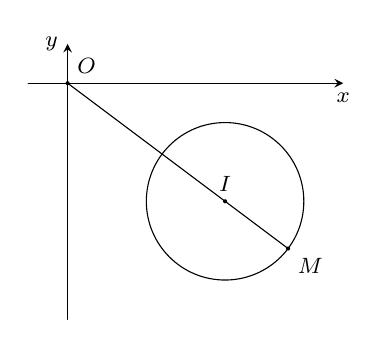
\begin{tikzpicture}[scale=0.5,>=stealth, font=\footnotesize, line join=round, line cap=round]
		\def\xmin{-1} \def\xmax{7}  \def\ymin{-6}  \def\ymax{1} 
%		\draw[color=gray!50,dashed] (\xmin,\ymin) grid (\xmax,\ymax);
		\draw[->] (\xmin,0)--(\xmax,0) node [below]{$x$};
		\draw[->] (0,\ymin)--(0,\ymax) node [left]{$y$};
		\clip (\xmin,\ymin) rectangle (\xmax,\ymax);

		\coordinate[label=above:{$I$}] (I) at (4,-3);
		\coordinate[label=above right:{$O$}] (O) at (0,0);
		\coordinate[label=below right:{$M$}] (M) at (5.6,-4.2);
		\draw (I) circle(2cm);
		\draw (O)--(M);
			\foreach \diem in {O,M,I}	\fill (\diem)circle(1.5pt);
\end{tikzpicture}}
}
\end{ex}



\Closesolutionfile{ans}

\begin{center}
	\textbf{PHẦN 2 - TỰ LUẬN}
\end{center}


\begin{bt}%[Dự án đề kiểm tra GHK2 NH22-23- Võ Thị Thùy Trang]%[0T7B3-2]
	Không sử dụng máy tính hãy giải phương trình và bất phương trình sau
	\begin{enumerate}
		\item $2 x^2+5 x+2 \leq 0$.
		\item $\sqrt{x^2+4 x-3}=2 x-1$.
	\end{enumerate}
\loigiai{
\begin{enumerate}
	\item $2 x^2+5 x+2 \leq 0$.
	   \begin{itemize}
		\item Ta có $2 x^2+5 x+2 =0 \Leftrightarrow \hoac{&x=-\dfrac{1}{2}\\&x=-2.}$
		\item Bảng xét dấu 
		\begin{center}
			\begin{tikzpicture}
				\tkzTabInit[nocadre=false,lgt=3.5,espcl=2,deltacl=0.6]
				{$x$ /0.9,$2x^2+5x+2$ /.6}
				{$-\infty$,$-2$,$-\dfrac{1}{2}$,$+\infty$}
				\tkzTabLine{,+,$0$,-,$0$,+,}
			\end{tikzpicture}
		\end{center}
  	  \end{itemize}
  	  Vậy tập nghiệm của bất phương trình là $S=\left[-2;-\dfrac{1}{2}\right]$.
\item Ta có 
\begin{eqnarray*}
\sqrt{x^2+4 x-3}=2 x-1& \Rightarrow &x^2+4x-3=4x^2-4x+1\\
& \Leftrightarrow & 3x^2-8x+4=0 \Leftrightarrow \hoac{&x=2\\&x=\dfrac{2}{3}.}
\end{eqnarray*}
Thay $ x=2 $ và $ x=\dfrac{2}{3} $ vào phương trình đã cho ta thấy thỏa mãn.\\
Vậy tập nghiệm của phương trình là $S=\left\lbrace\dfrac{2}{3};2\right\rbrace $.
\end{enumerate}
}
\end{bt}
\begin{bt}%[Dự án đề kiểm tra GHK2 NH22-23- Võ Thị Thùy Trang]%[0T9B2-2]%[0T9B2-6]
	Trong mặt phẳng tọa độ $Oxy$, cho $\triangle ABC$ biết $A(2;3)$, $B(4 ;-1)$ và $C(5;1)$.
	\begin{enumerate}
		\item Viết phương trình tổng quát của đường cao $AH$ của $\triangle A
		BC$.
		\item Tìm tọa độ điểm $D$ sao cho tứ giác $A B C D$ là hình bình hành.
	\end{enumerate}
	\loigiai{
			\begin{enumerate}
			\item \immini{Ta có $AH\perp BC$ nên $\overrightarrow{BC}=\left(1;2\right)$ là một véc-tơ pháp tuyến của đường cao $AH$.\\
				Phương trình đường cao $AH$ là \[1(x-2)+2(y-3)=0 \Leftrightarrow x+2y-8=0.\]}
				{
				\begin{tikzpicture}[scale=.8, font=\footnotesize, line join=round, line cap=round, >=stealth]
	\def\a{3}
	\path (2,3) coordinate (A)
	(0,0) coordinate (B)
	(6,0) coordinate (C)
    (2,0) coordinate (H)
	;
	\draw (A)--(B)--(C)--cycle (A)--(H);
	\foreach \f/\g in {A/90,B/180,C/0,H/-90}{
	\draw[fill=black] (\f) circle (1pt) node[shift={(\g:7pt)},font=\scriptsize]{$ \f $};
	\draw pic[draw=black, angle eccentricity=2, angle radius=0.25cm]
	{right angle=A--H--C};
		}	
	\end{tikzpicture}
				}
			\item Tứ giác $ABCD$ là hình bình hành khi và chỉ khi \[ \overrightarrow{AD}=\overrightarrow{BC} \Leftrightarrow \heva{&x_D-x_A=x_C-x_B\\&y_D-y_A=y_C-y_B} \Leftrightarrow \heva{&x_D=x_A+x_C-x_B=3\\&y_D=y_A+y_C-y_B=5.}\]
			Vậy $D(3;5)$.
		\end{enumerate}
	}
\end{bt}
